\chapter{Introduzione}
\section{La bioinformatica}
    La \textbf{bioinformatica} è una disciplina che combina la \textbf{biologia}, l'\textbf{informatica} e la \textbf{statistica} per analizzare, elaborare e interpretare i dati biologici utilizzando \emph{strumenti computazionali}. Con l'avvento delle tecnologie di sequenziamento di \emph{DNA} e \emph{RNA} ad alta velocità il volume di dati biologici generati è aumentato a dismisura, rendendo necessario integrare un approccio computazionale nelle metodologie di analisi biologica. La bioinformatica risulta quindi indispensabile per gestire, analizzare e trarre informazioni significative dall'enorme quantità di dati che viene generata.
    
    Questa disciplina di recente nascita svolge un ruolo fondamentale in molteplici ambiti della biologia, trovando un'applicazione a diverse componenti della letteratura informatica sviluppata negli anni passati. Attraverso l'uso di algoritmi, modelli statistici e metodi computazionali, la \textbf{bioinformatica} consente, tra le altre cose, di analizzare sequenze genetiche, identificare geni, annotare genomi, studiare l'evoluzione e predire la struttura delle proteine.
    
    In particolare, una componente che si dimostra cruciale in queste specifiche applicazioni è l'\textbf{allineamento di sequenze}, risultando uno strumento fondamentale per analizzare le similarità e le differenze tra le sequenze biologiche.

\section{Applicazioni dell'allineamento di sequenze}
    Uno dei principi ampiamenti riconosciuti nella \textbf{biologia molecolare}, che si pone come uno dei pilastri di questa disciplina, è il seguente:
    \begin{quote}
         Nelle \textbf{sequenze biomolecolari} (\emph{DNA, RNA o sequenze amminoacide}), \textbf{un'alta similarità delle sequenze} di solito implica \textbf{significative similarità funzionali e/o strutturali}. \cite{Gusfield}
    \end{quote}
    Il fatto che due sequenze biomolecolari presentino un'alta similarità significa che esse condividono una notevole quantità di informazioni genetiche o strutturali. Questo può indicare che le due sequenze derivino da organismi strettamente correlati o che svolgano funzioni simili.

    In particolare, la \textbf{similarità funzionale} può indicare che le sequenze condividono una specifica attività biologica o svolgono un ruolo simile all'interno di un processo biologico, mentre la \textbf{similarità strutturale} si riferisce alla conservazione della struttura tridimensionale delle biomolecole: sequenze con alta similarità strutturale possono indicare comformazioni simili per le proteine corrispondenti. Tuttavia, è importante notare che non sempre la similarità delle sequenze garantisce una funzionalità o struttura identica: esistono infatti diversi casi in cui questo non accade. 
    
    Di conseguenza, l'allineamento di sequenze risulta fondamentale nella ricerca di \textbf{regioni conservate}, che sono segmenti di sequenze simili o addirittura identiche: esse spesso indicano l'esistenza di una funzione biologica comune o di una relazione evolutiva condivisa. Un esempio sono le sequenze proteiche, in cui regioni conservate possono rivelare la presenza di motivi strutturali o di siti attivi importanti per la loro funzione.
    
    Un'altra applicazione importante dell'allineamento è l'\textbf{identificazione di variazioni o mutazioni}. Durante l'evoluzione, le sequenze nucleotidiche subiscono cambiamenti a livello genetico (ad esempio \emph{mutazioni puntiformi}, \emph{inserzioni} o \emph{delezioni}). L'allineamento mette in evidenza le differenze tra le sequenze, permettendo di individuare queste mutazioni e di studiare il loro impatto sulla struttura e sulla funzione delle biomolecole. Un esempio di questa applicazione è il campo della ricerca sulle malattie genetiche, dove l'allineamento di sequenze genomiche può rivelare varianti genetiche associate a condizioni patologiche.
    
    Inoltre, i risultati forniti dall'allineamento vengono utilizzati anche all'interno di altri campi della bioinformatica: nella costruzione degli \textbf{alberi filogenetici}, utilizzati per rappresentare storie e relazioni evolutive, vengono usati gli allineamenti di sequenze nucleotidiche per stimare la \emph{distanza evolutiva} di specie diverse.

\section{Tecnologie di sequenziamento}
    Uno dei principali motivi dei progressi nei campi della biologia e della genetica sono le \textbf{tecnologie di sequenziamento}, un insieme di metodi e strumenti utilizzati per determinare l'ordine esatto dei nucleotidi (A, C, G, T) all'interno di una molecola di \emph{DNA} o \emph{RNA}. Il loro sviluppo ha consentito la generazione di quantità sempre crescenti e di maggior qualità di dati genomici, in modo rapido ed efficiente.

\clearpage

\begin{figure}[ht]
%\hspace*{-2cm}
\centering
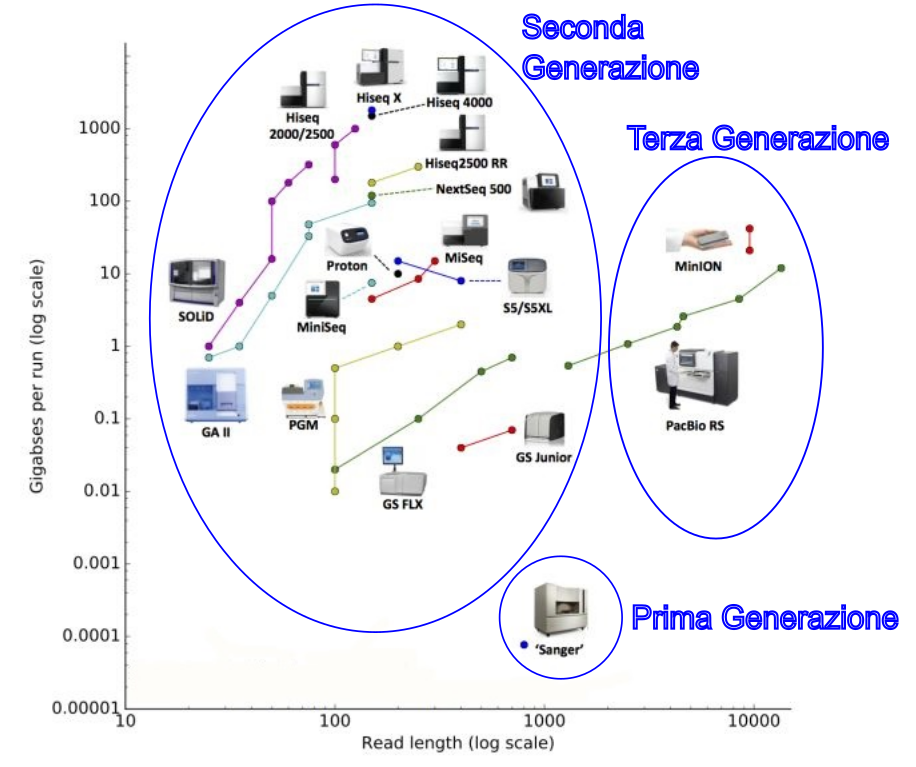
\includegraphics[width=1\linewidth]{images/sequencing_technologies.png} 
\caption[Tecnologie di sequenziamento]{Suddivisione delle \emph{tecnologie di sequenziamento} in generazioni.}
\label{fig:tecnologie_sequenziamento}
\end{figure}
\vspace{30pt}
\noindent
Come si vede dalla figura \ref{fig:tecnologie_sequenziamento}, è possibile dividere le \textbf{tecnologie di sequenziamento} in \textbf{tre generazioni}:
\begin{itemize}
    \item \textbf{Prima generazione}:
    tecnologie conosciute anche come \emph{sequenziamento  Sanger}, sono state usate nel progetto \emph{Genoma Umano} per riuscire a ricostruire l'intero patrimonio genetico di un essere umano; producono sequenze di \emph{lunghezza} pari a circa 1000 nucleotidi con un \emph{throughput}\footnote{Per \emph{throughput} si intende la quantità di dati prodotta in un determinato lasso di tempo (nella figura \ref{fig:tecnologie_sequenziamento} Gigabasi per esecuzione).} limitato, insieme a un \emph{tasso di errore} del $6\%$ circa;

    \item \textbf{Seconda generazione}:
    la classe di tecnologie più sviluppata, hanno come punto di forza un \emph{elevato throughput}, mantenendo anche un \emph{basso tasso di errore} ($<1\%$) e \emph{lunghezza delle sequenze} abbastanza variabile, sempre però al di sotto delle 1000 bp\footnote{bp sta per \emph{base pair}, che indica una coppia di nucleotidi; viene usata come unità di misura per la lunghezza delle sequenze generitiche.} del \emph{sequenziatore Sanger}; hanno però il limite di produrre \emph{errori sistematici} sempre dello stesso tipo; 

    \item \textbf{Terza generazione}:
    classe ancora in forte sviluppo, si concentrano sulla produzione di sequenze di \emph{elevata lunghezza} (quasi 10000 nucleotidi per sequenza), mantenendo un \emph{throughput} abbastanza elevato. Producono \emph{errori} con un tasso piuttosto elevato (più del $10\%$), che sono però distribuiti in maniera \emph{casuale}. 
\end{itemize}
La tabella \ref{tab:errori_sequenziatori} riporta in maniera strutturata le caratteristiche delle varie generazioni di \emph{tecnologie di sequenziamento}.

\vspace{30pt}
\begin{table}[h]
    \centering
    \begin{tabular}{|c|c|c|c|c|}
        \hline
            \multicolumn{5}{|c|}{\textbf{Tecnologie di sequenziamento}} \\
        \hline
            \textbf{Generazione} & \textbf{Sequenze} & \textbf{Throughput} & \textbf{Tasso di errore} & \textbf{Tipo di errore} \\
        \hline
            Prima & $\approx 1000$ & $< 0.01$ & $\approx 6\%$ & Casuale \\
        \hline
            Seconda & tra 50 e 1000 & fino a $18000$ & $<1\%$ & Sistematico \\
        \hline
            Terza & $\approx 10000$ & $\approx 10$ & $>10\%$ & Casuale \\
        \hline
    \end{tabular}
    \caption{Caratteristiche delle varie generazioni di tecnologie di sequenziamento; il \emph{throughput} è misurato in \emph{Gb/day} e la \emph{lunghezza} delle sequenze in \emph{bp}.}
    \label{tab:errori_sequenziatori}
\end{table}

\section{Obiettivo dello stage}
    L'obiettivo dello stage era quello di effettuare uno studio approfondito dell'algortimo \textbf{\textit{wavefront}}, un nuovo approccio basato sulla \emph{programmazione dinamica} che permette di calcolare la \textbf{distanza di edit} in tempo proporzionale al valore della distanza stessa (capitolo \ref{section:wfa}). 
    
    In particolare, l'obiettivo finale era quello di integrare l'approccio \textbf{\textbf{wavefront}} all'interno di \href{https://github.com/AlgoLab/RecGraph}{\textbf{\textit{RecGraph}}} \cite{Recgraph}, un tool precedentemente sviluppato che permette di effettuare numerosi tipi di allineamenti tra un \emph{grafo} e una \emph{sequenza}, in particolare un allineamento che permette di individuare fino a una \emph{ricombinazione} all'interno del genoma rappresentato nel grafo. 
    
    Nella prima parte del percorso ci si è concentrati sullo studio dell'algoritmo, partendo da una sua applicazione su due sequenze per poi cercare di generalizzarlo su strutture dati più complesse (\textbf{grafi di sequenza} e \textbf{grafi di variazione}).
    
    In una seconda parte si è passati all'implementazione di un prototipo (nel linguaggio \href{https://www.rust-lang.org/it}{\textbf{\textit{Rust}}}) che utilizzasse l'algoritmo \textbf{\textit{wavefront}} per effettuare un allineamento tra \textbf{grafi di variazione} e \textbf{sequenze} e che permettesse di migliorare le capacità computazionali di \textbf{\textit{RecGraph}}, rendendo possibile l'utilizzo di istanze di grafi di dimensioni sempre maggiori.  